%%%%%%%%%%%%%%%%%%%%%%%%%%%%%%%%%%%%%%%%%%%%%%%%%%%%%%%%%%%%%%%%%%%%%%%%%%%

\documentclass{standalone}

\usepackage{amsmath}
\usepackage{mathptmx}
\usepackage{pgfplots}
\usetikzlibrary{external}
\tikzexternalize{population-sweden}
\pgfplotsset{compat=1.16}

%% IEEE uses Times Roman font, so we'll default to Times.
%% These three commands make up the entire times.sty package.
\renewcommand{\rmdefault}{ptm}
\renewcommand{\ttdefault}{pcr}
\normalfont\selectfont

\begin{document}

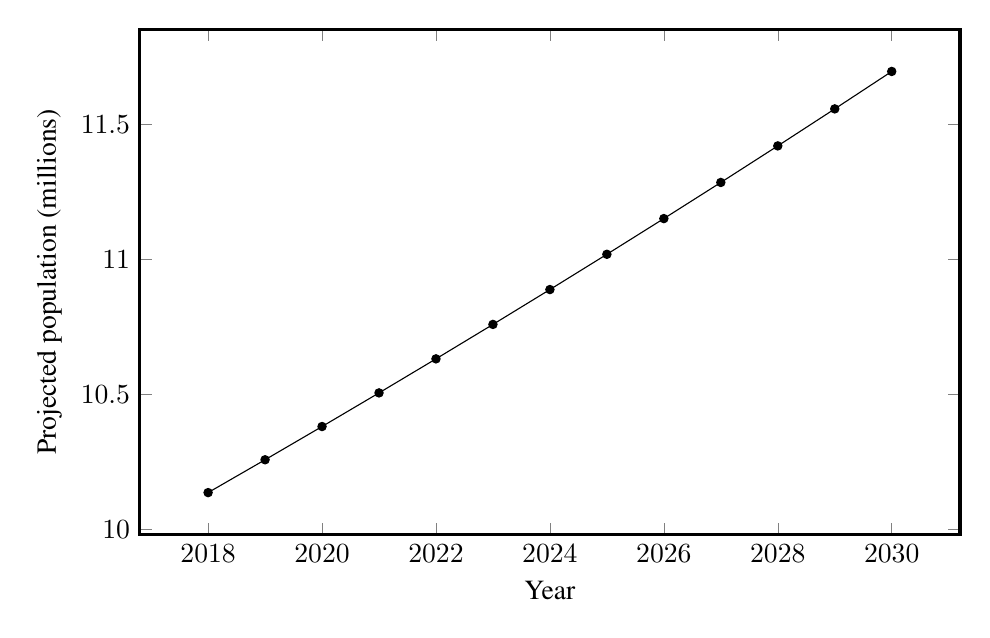
\begin{tikzpicture}
\tikzset{%%
  every mark/.append style={scale=1.0},%%
  scale=1.0%%
}
\pgfplotsset{%%
  every axis/.append style={font=\normalsize}%%
}
%%
\begin{axis}[%%
  axis line style=very thick,%%
  dotStyle/.style={mark size=1.5,black,mark color=black,mark=*},%%
  enlargelimits=true,%%
  height=8cm,%%
  width=12cm,%%
  %% x axis
  xlabel={\normalsize Year},%%
  xtick={2018,2020,2022,2024,2026,2028,2030},%%
  xticklabels={$2018$,$2020$,$2022$,$2024$,$2026$,$2028$,$2030$},%%
  %% y axis
  ylabel={\normalsize Projected population~(millions)}%%
]
%%
%%
\addplot[dotStyle] coordinates {
  (2018, 10.135303)
  (2019, 10.256927)
  (2020, 10.380010)
  (2021, 10.504570)
  (2022, 10.630625)
  (2023, 10.758192)
  (2024, 10.887291)
  (2025, 11.017938)
  (2026, 11.150153)
  (2027, 11.283955)
  (2028, 11.419363)
  (2029, 11.556395)
  (2030, 11.695072)
};
\end{axis}
\end{tikzpicture}

\end{document}
